\section{Auswertung}
\label{sec:Auswertung}
% \subsection{Fehlerrechnung}
% Der Mittelwert einer physikalischen Größe $a$ mit $N$ Einzelmesswerten ist gegeben durch
% \begin{equation}\label{eq:mean}
%     \overline{x}=\frac{1}{N}\sum_{i=1}^Na_\text{i}\,.
% \end{equation}
% Die Standardabweichung eines Mittelwerts zu einer physikalischen Größe a bestimmt sich mit
% \begin{equation}\label{eq:std}
%     \Delta{x}=\sqrt{\frac{1}{N(N-1)}\sum_{i=1}^N\left(a_\text{i}-\overline{x}\right)}\,.
% \end{equation}

% \begin{table}[H]
%   \centering
%   \caption{}
%   \label{tab:}
%   \begin{tabular}{S[table-format=2.1] S[table-format=4] S[table-format=2.1] S[table-format=4]S[table-format=3]S[table-format=2.1]}
%       \toprule
%       {}&{}&{}&{}&{}\\
%       \midrule
      
%       \bottomrule
%   \end{tabular}
% \end{table}

% \begin{figure}[H]
%   \centering
%   \includegraphics{build/}
%   \caption{.}
%   \label{fig:}
% \end{figure}

\subsection{Kalibrierung des Detektors} \label{sec:kalibrierung}
Um den Germaniumdetektor zu kalibrieren wird eine $^{152}\text{Eu}$-Probe verwendet und dessen Spektrum gemessen.
Die Messung dauerte $t = 3634 \, \si{\second}$.
Die Energie der Gamma-Quanten wird dabei aus der Literatur entnommen. 
Des Weiteren wurde eine Untergrundmessung durchgeführt und nach einer Normierung von der $^{152}\text{Eu}$-Messung abgezogen.
Die Untergrundmessung dauerte $t = 78108 \, \si{\second}$.
Die Normierung bezieht sich auf die unterschiedlichen Messzeiten von Europium- und Untergrundmessung.
Das Spektrum der Untergrundstrahlung ist in Abbildung \ref{fig:untergrund} dargestellt.

\begin{figure}[H]
  \centering
  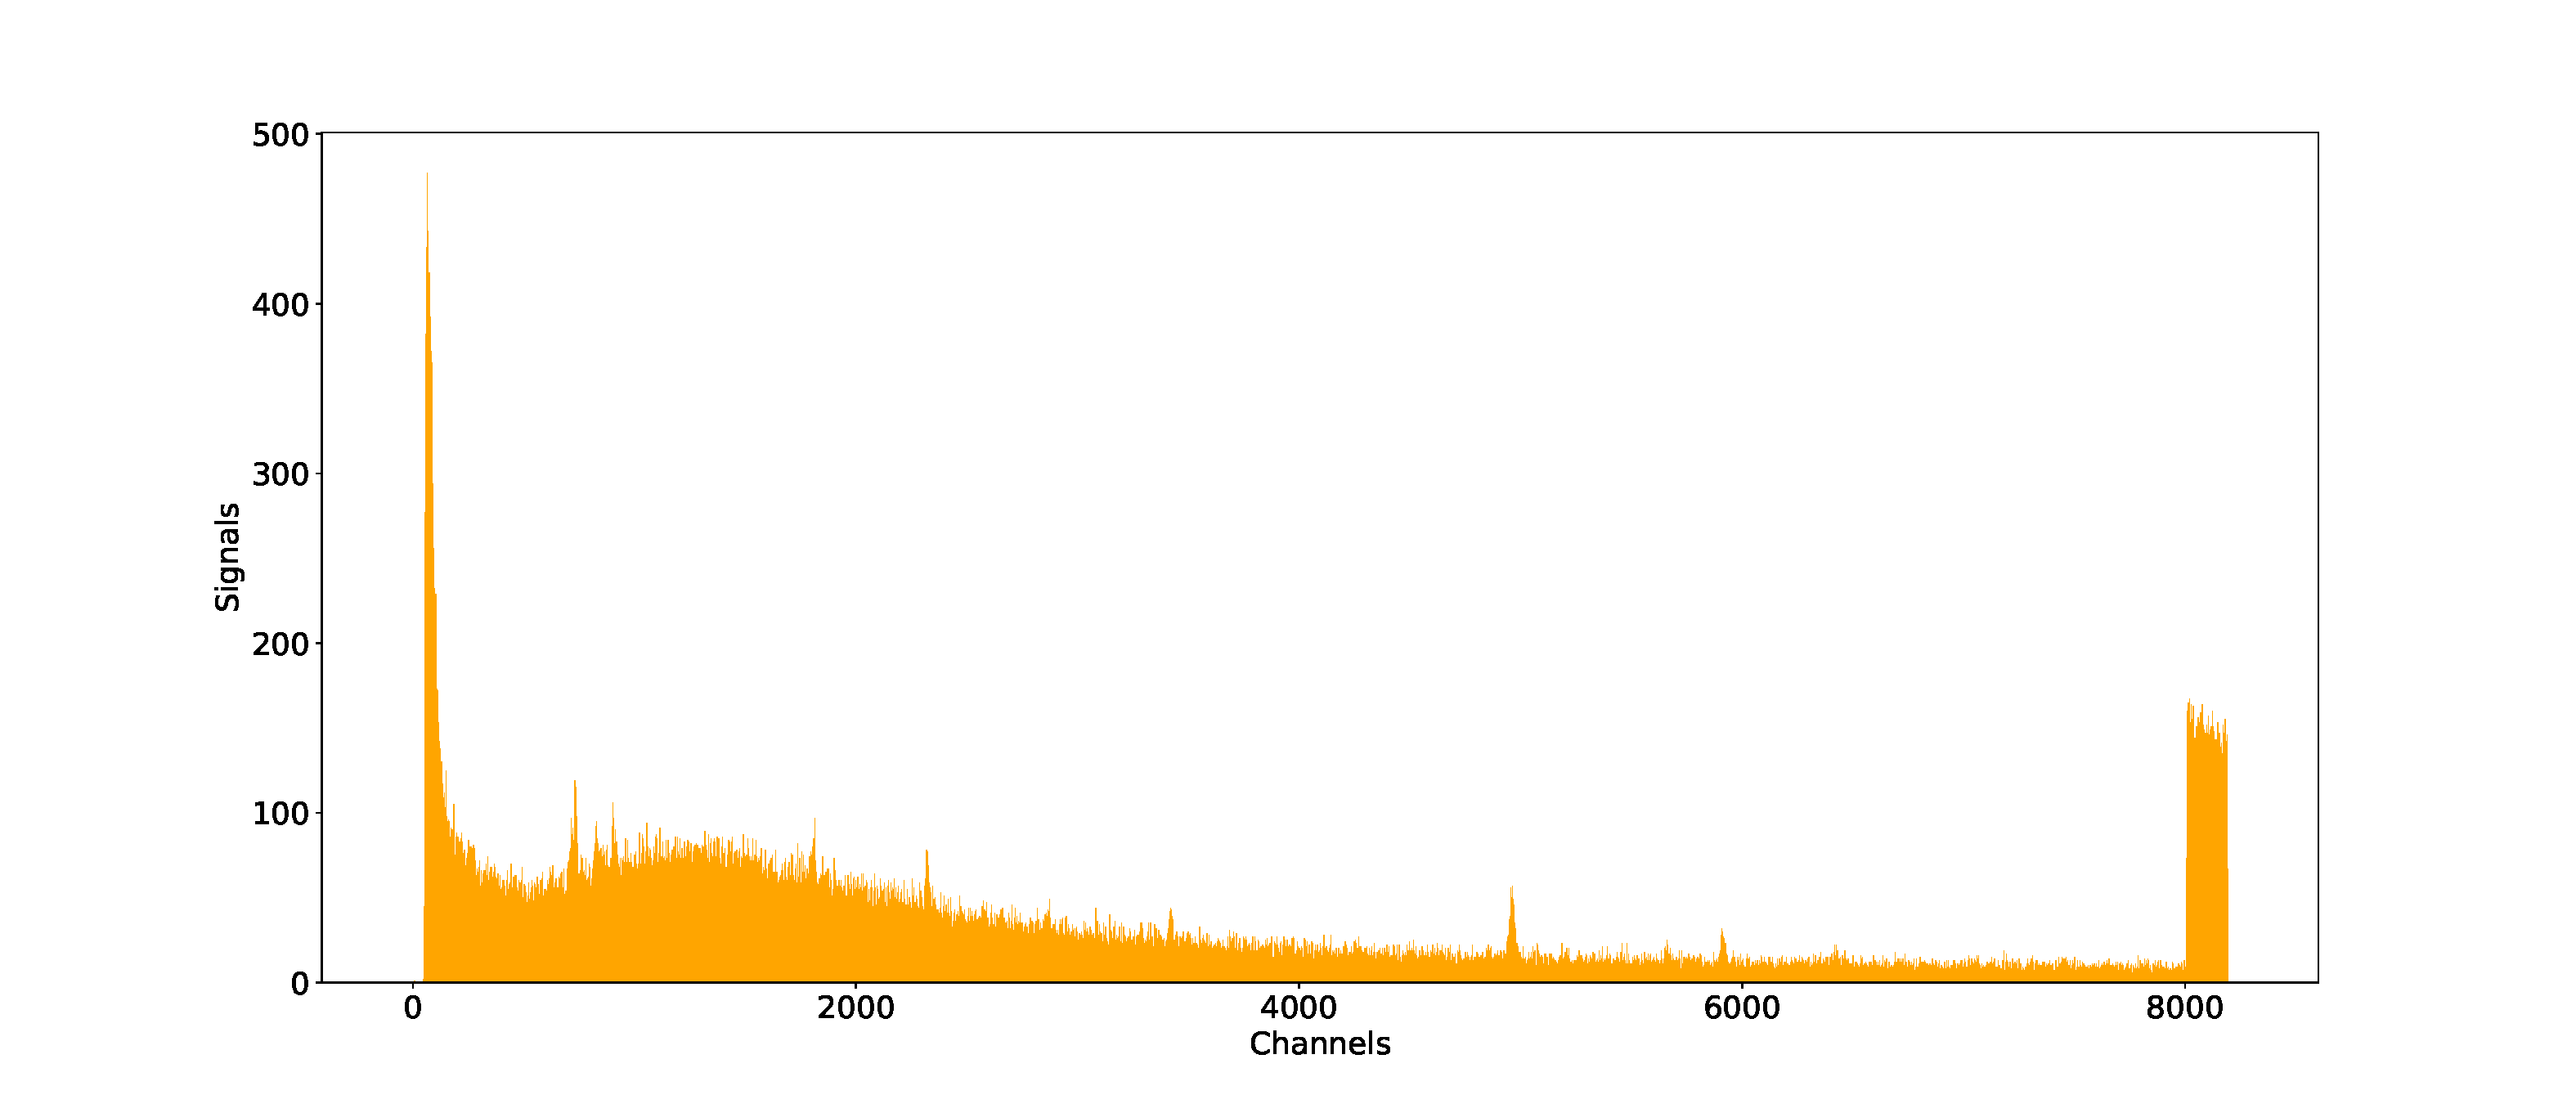
\includegraphics[width=\textwidth]{../plots/Untergrund.pdf}
  \caption{Spektrum der Untergrundstrahlung.}
  \label{fig:untergrund}
\end{figure}

Um den Kanälen des Detektors eine Energie zuzuordnen, wurden zunächst die prominentesten Peaks des $^{152}\text{Eu}$-Spektrums identifiziert 
und mit den wahrscheinlichsten Emissionsenergien aus der Literatur verglichen.
Die Peaks wurden mit Hilfe von \texttt{find\_peaks} der python-Bibliothek \texttt{scipy} \cite{scipy} 
identifiziert.
Die Peaks und die zugehörigen Energien sind in Tabelle \ref{tab:eu} aufgeführt und in Abbildung \ref{fig:eu} dargestellt.

\begin{figure}[H]
  \centering
  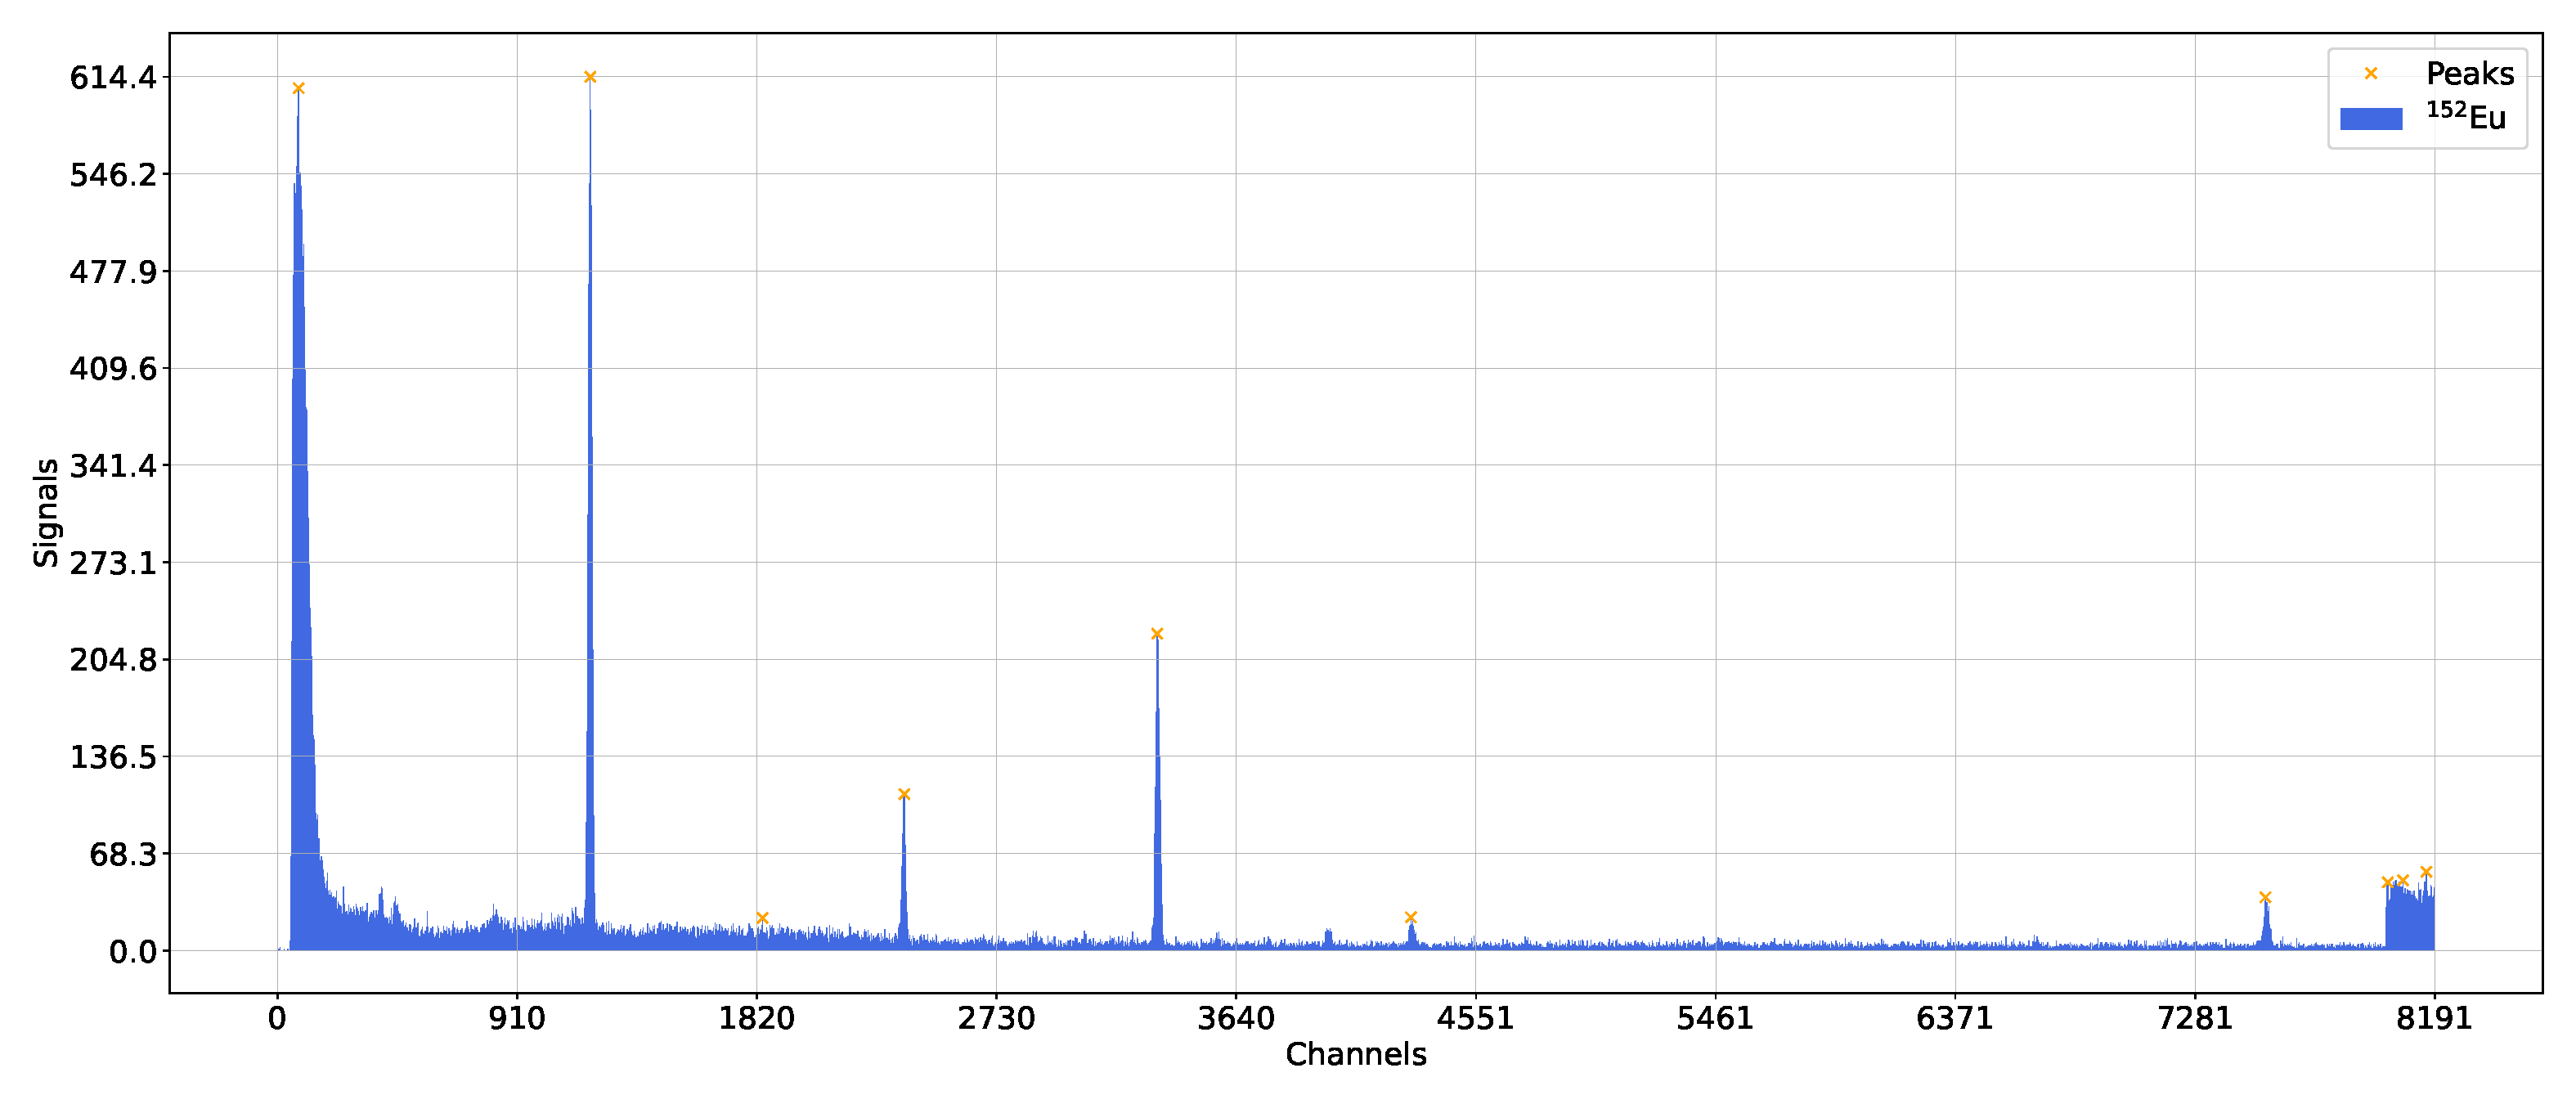
\includegraphics[width=\textwidth]{../plots/Europium-Peaks.pdf}
  \caption{Spektrum der $^{152}\text{Eu}$-Probe und dessen prominentesten Peaks.}
  \label{fig:eu}
\end{figure}

\begin{table}[H]
  \centering
  \caption{Energien und Wahrscheinlichkeiten der Vollenergiepeaks der $^{152}\text{Eu}$-Probe sowie die zugenorndeten Kanäle.}
  \label{tab:eu}
  \begin{tabular}{S S[table-format=4] S[table-format=3.1] S}
      \toprule {$E_\text{Lit} / \si{\kilo\electronvolt}$} & {$P_\text{Lit} /\si{\percent}$} & {Kanal} & {Counts}\\
      \midrule
      121.7817& {28.41 \pm 0.13}&1187&{10137.2 \pm 100.7}\\
      344.2785& {26.59 \pm 0.12}&2380&{1767.1 \pm 42.0} \\
      778.9045& {12.97 \pm 0.06}&3340&{3900.4 \pm 62.5} \\
      964.079 & {14.5 \pm 0.06} &3985&{234.3 \pm 15.3} \\
      1112.076& {13.41 \pm 0.06}&4303&{388.6 \pm	34} \\
      1408.013& {20.85 \pm 0.08}&7548&{752.8 \pm 27.4} \\
      \bottomrule
  \end{tabular}
\end{table}

Für alle Peaks wurde eine Gaußfunktion der Form 
\begin{equation}
  f(x) = \frac{a}{\sqrt{2*\pi*\sigma^2}} \cdot \exp\left(-\frac{(x-\mu)^2}{2\sigma^2}\right) \label{eq:gauss}
\end{equation}
gefittet und anhand dessen der Inhalt der Peaks durch eine Integration der Gaußfunktion bestimmt.
Lediglich für den Peak bei der Kanalnummer 4303 konnte keine passende Gaußfunktion gefunden werden, sodass der Inhalt händisch bestimmt wurde.
Die Ergebnisse sind in Tabelle \ref{tab:eu} aufgeführt.
Die Kalibrierung erfolgt durch eine lineare Regression der Form

\begin{equation}
  E = a \cdot K + b
\end{equation}
und stellt damit eine Beziehung zwischen Kanalnummer $K$ und Energie $E$ her.
Die Parameter der Regression betragen

\begin{align*}
    a &= {0.228334 \pm 0.0} \, \si{\kilo\electronvolt} \\
    b &= -148.659709 \pm 0.000593 \, \si{\kilo\electronvolt} \, 
\end{align*}

und werden im weiteren Verlauf zur Energiebestimmung der Peaks verwendet.
Der Fit ist in Abbildung \ref{fig:kalibrierung} dargestellt.

\begin{figure}[H]
  \centering
  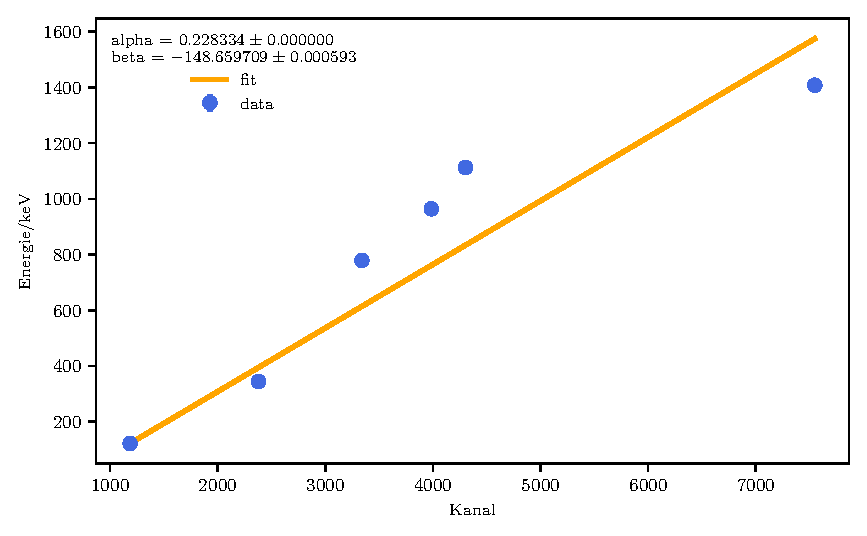
\includegraphics[width=\textwidth]{../plots/Europium-Fit.pdf}
  \caption{Ausgleichsfunktion der gemessenen Energien und der zugeordneten Kanäle.}
  \label{fig:kalibrierung}
\end{figure}

\subsection{Vollenergie-Detectionswahrscheinlichkeit}
Die Vollenergie-Detectionswahrscheinlichkeit $Q$ ist durch 
\begin{equation}
  Q = \frac{4 \pi N}{\Omega A P t}
\end{equation}
gegeben.
Dabei ist $N$ die Anzahl der gemessenen Photonen, $\Omega$ der Raumwinkel, $A$ die Aktivität, $P$ die Emissionswahrscheinlichkeit und $t$ die Messzeit.
Die Werte für die Emissionswahrscheinlichkeit und die Anzahl der gemessenen Photonen sind in Tabelle \ref{tab:eu} aufgeführt.
Der Raumwinkel des Germaniumdetektors beträgt
\begin{equation}
  \frac{\Omega}{4\pi} =\frac{1}{2}\left(1-\frac{a}{\sqrt{a^2+r^2}}\right) 
\end{equation}
mit den Werten 
\begin{align*}
  a &= 2.25 \, \si{\centi\meter} \\
  r &= 8.52 \, \si{\centi\meter} \, .
\end{align*}
Somit ergibt sich ein Raumwinkel von $\Omega = 0.01657$.
Die Aktivität der $^{152}\text{Eu}$-Probe betrug am Tag der Produktion (01.10.2000) $A_0 = (4130 \pm 60) \, \si{\becquerel}$.
Die Aktivität $A$ zum Messzeitpunkt wird durch
\begin{equation}
  A = A_0 \cdot \exp\left(-\frac{\ln(2)}{t_{1/2}} \cdot t\right)
\end{equation}
berechnet.
Mit einer Halbwertszeit von $t_{1/2} = 13.522$ Jahre ergibt sich am Tag der Messung (21.10.2024) 
eine Aktivität von $A = ( 1203 \pm 17 ) \, \si{\becquerel}$.
Die berechnete Vollenergie-Detectionswahrscheinlichkeit ist in der Tabelle \ref{tab:fedp} aufgeführt.

\begin{table}
    \centering
    \caption{Vollenergie-Detectionswahrscheinlichkeit der $^{152}\text{Eu}$-Probe.}
    \label{tab:fedp}
    \begin{tabular}{S S[table-format=1.5]}
        \toprule {$E_\text{Lit} / \si{\kilo\electronvolt}$} & {$Q / \si{\percent}$} \\
        \midrule
        121.7817&{0.06186	\pm 0.00112}\\
        344.2785&{0.01152	\pm 0.00033}\\
        778.9045&{0.05214	\pm 0.00115}\\
        964.079 &{0.0028	\pm 0.00019}\\
        1112.076&{0.00502	\pm 0.00045}\\
        1408.013&{0.00626	\pm 0.00025}\\
        \bottomrule
    \end{tabular}
\end{table}

Die Werte aus der Tabelle \ref{tab:fedp} sind in Abbildung \ref{fig:fedp} dargestellt.
Des Weiteren wurde die Energieabhängigkeit der Vollenergie-Detektionswahrscheinlichkeit untersucht und mit
\begin{equation}
  \label{eq:Q-fit}
  Q(E) = a \cdot E^{b}
\end{equation}
gefittet.
Die Parameter des Fits betragen
\begin{align*}
  a &= 25.8180 ± 3.2159\\
  b &= -1.2758 \pm 0.2262.
\end{align*}

\begin{figure}[H]
  \centering
  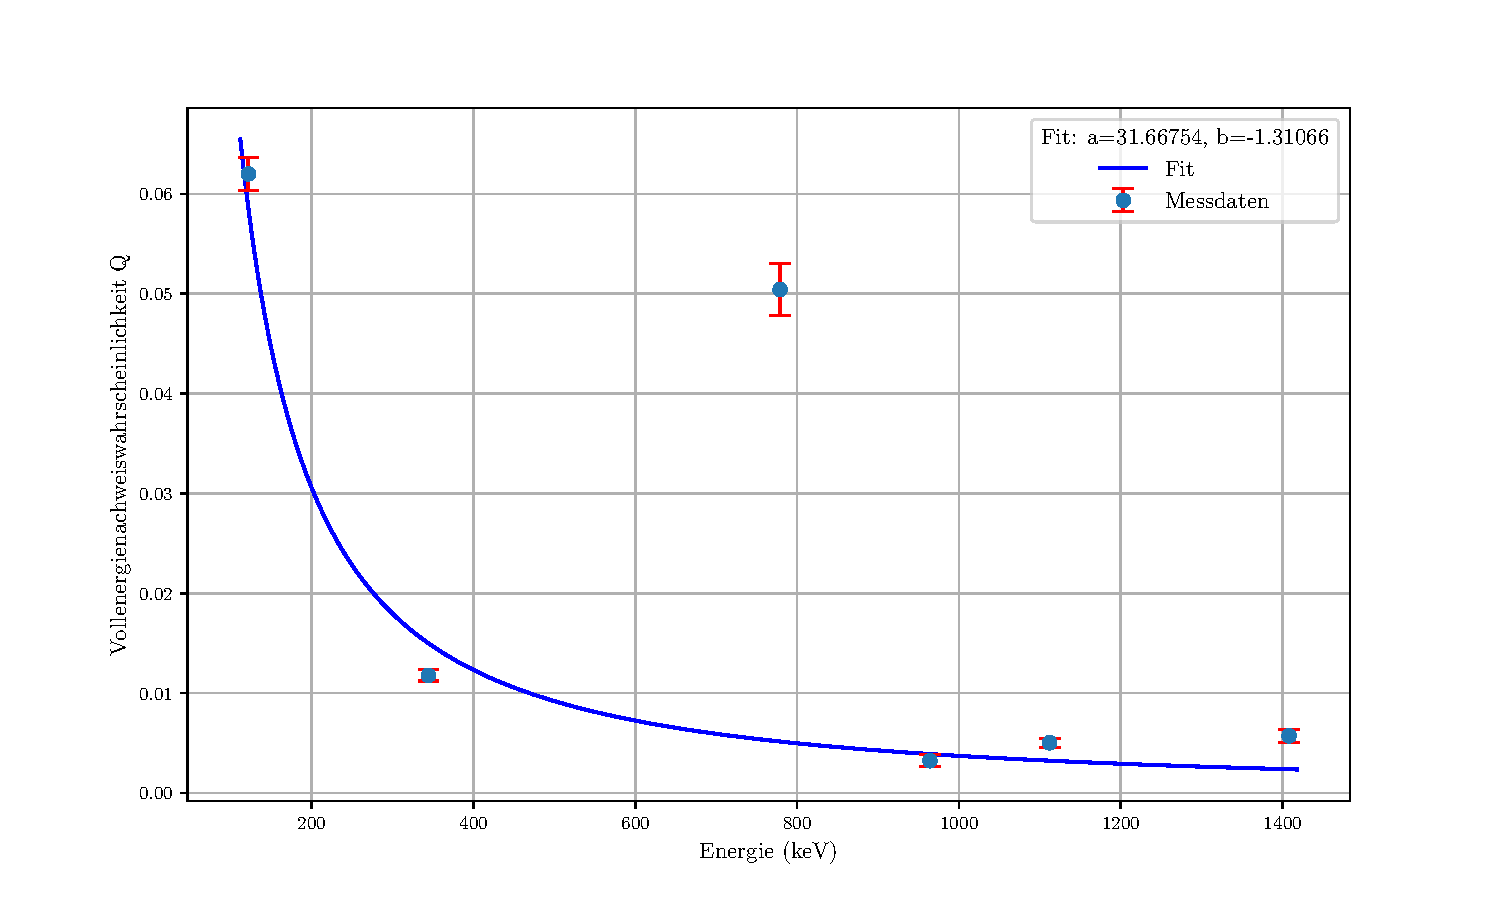
\includegraphics[width=\textwidth]{../plots/energie_vs_Q.pdf}
  \caption{Effizienz des Germaniumdetektors in Abhängigkeit der Energie.}
  \label{fig:fedp}
\end{figure}

\subsection{Untersuchung eines monochromatischen Gamma-Spektrums}
Das monochromatische Gamma-Spektrum des $^{137}\text{Cs}$-Strahlers ist in Abbildung \ref{fig:cs} dargestellt.
Die Messung dauerte $t = 3546 \, \si{\second}$.
Zu erkennen ist der Vollenergiepeak, die Compton-Kante und der Rückstreupeak. 
Zwischen der Compton-Kante und dem Rückstreupeak ist ein Compton-Kontinuum zu erkennen.

\begin{figure}[H]
  \centering
  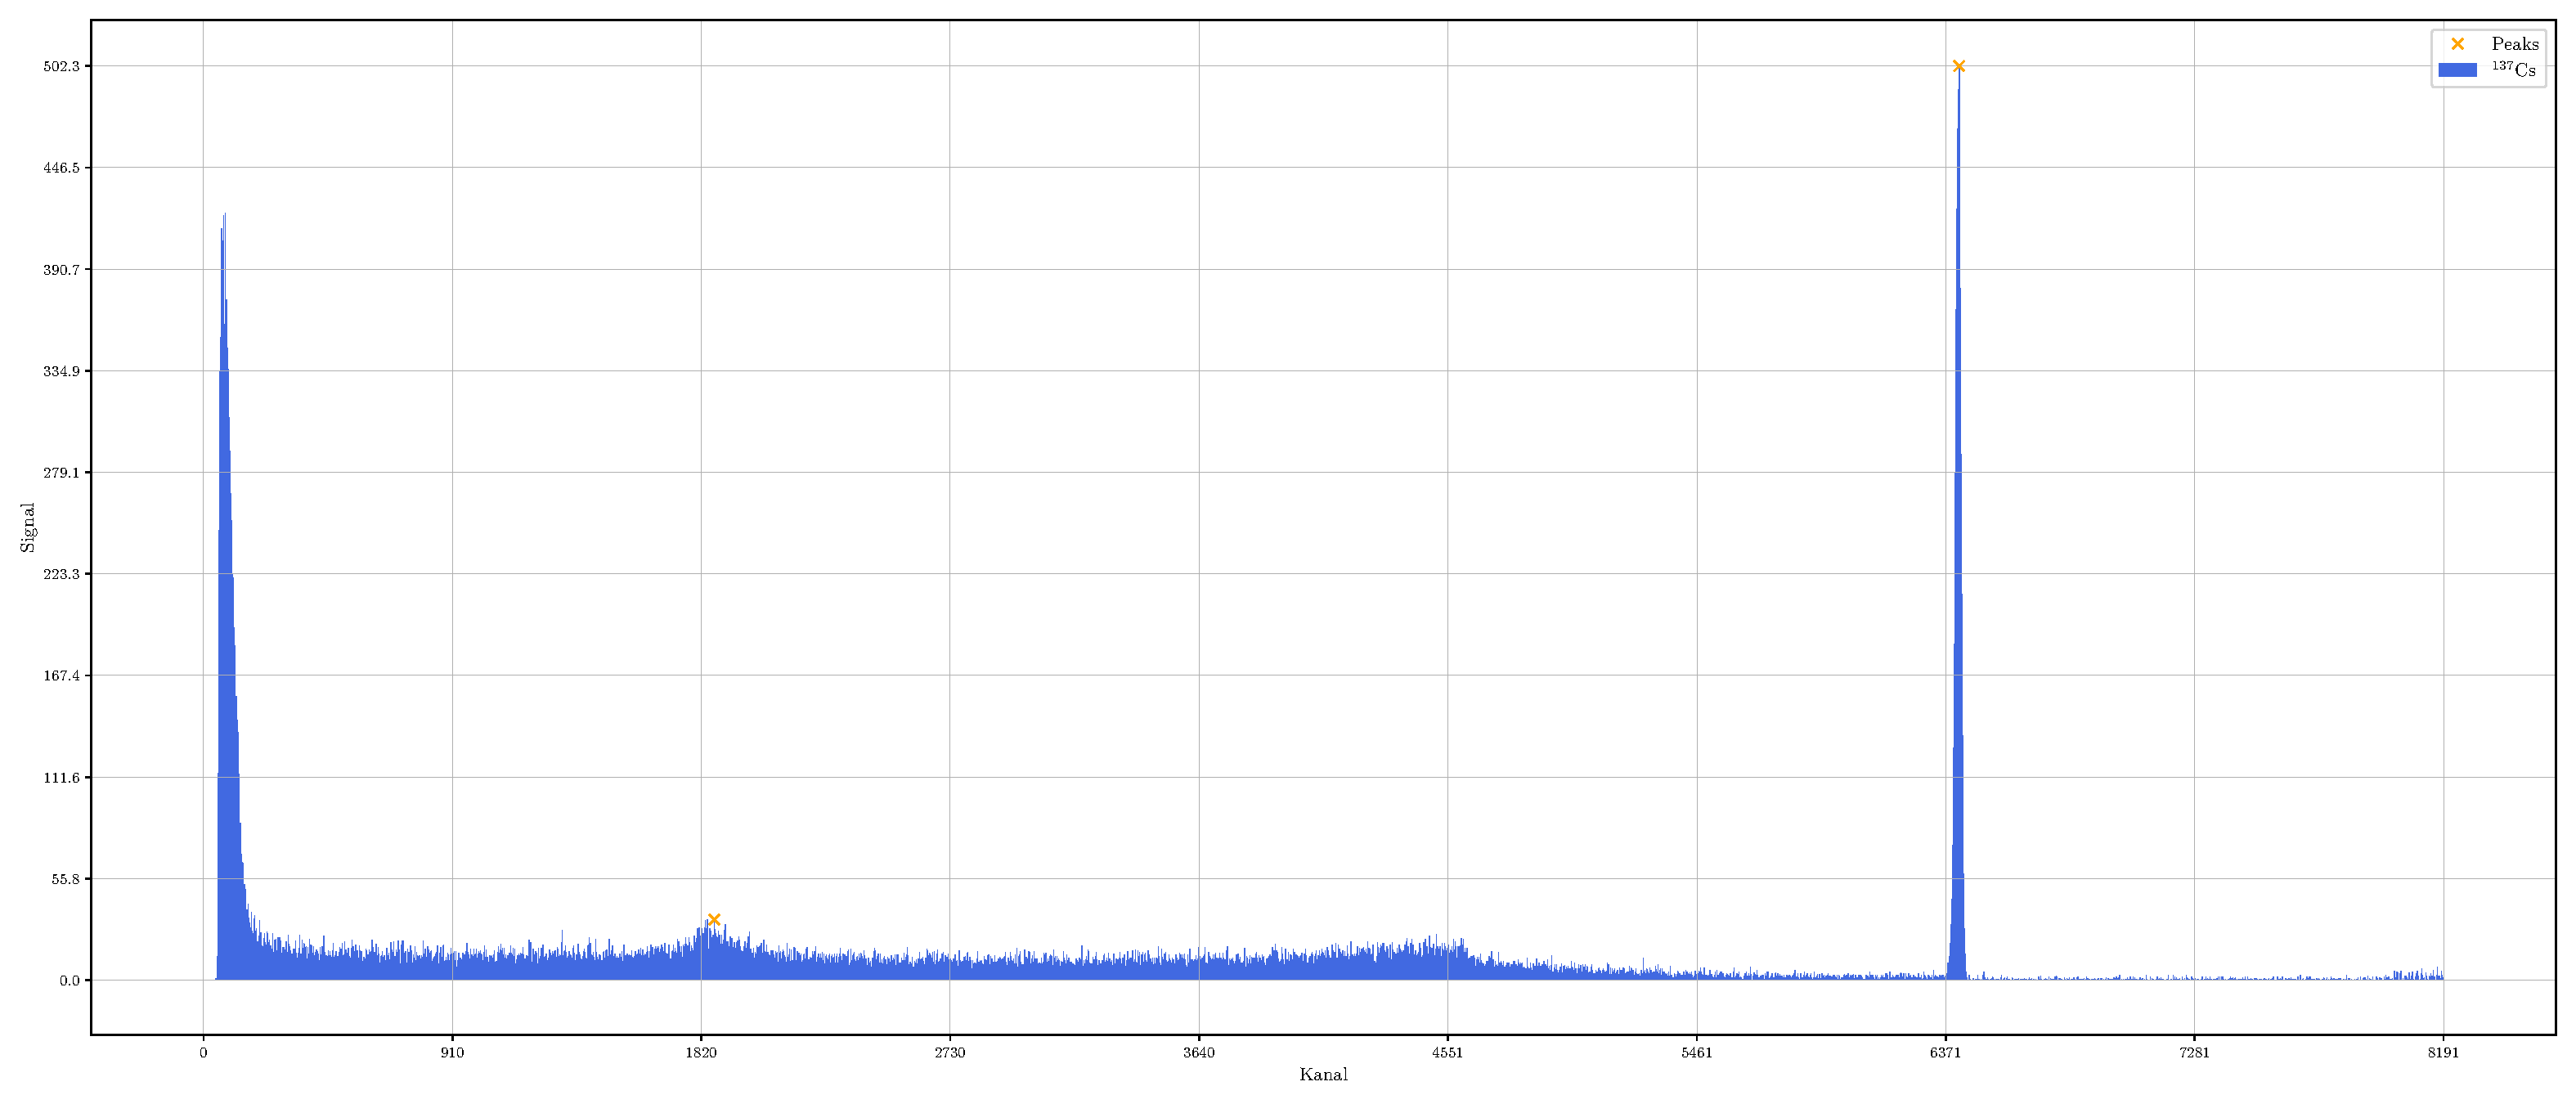
\includegraphics[width=\textwidth]{../plots/Caesium-Peaks.pdf}
  \caption{Spektrum des $^{137}\text{Cs}$-Strahlers.}
  \label{fig:cs}
\end{figure}

Die Position des Vollenergiepeaks und des Rückstreupeaks wurden wie in \ref{sec:kalibrierung} beschrieben bestimmt.

\subsubsection{Bestimmung der Halb- und Zehntelwertsbreite}
Demnach befindet sich der Vollenergiepeak bei Kanal 6420 und der Rückstreupeak bei Kanal 1868.
Des Weiteren wurde für den Vollenergiepeak eine Gaußfunktion \ref{eq:gauss} gefittet und der Inhalt des Peaks bestimmt.
Die Parameter der nichtlinearen Regression betragen
%A = (1.157+/-0.011)e+04, mu = 6415.86+/-0.09, sigma = 9.67+/-0.07
\begin{align*}
  a &= 1157 \pm 11 \\
  \mu &= 6415.86 \pm 0.09 \\
  \sigma &= 9.67 \pm 0.07 \, .
\end{align*}
Zusätzlich wurden die Halbwertsbreite und die Zehntelwertsbreite des Vollenergiepeaks bestimmt.
Dabei gibt die Halbwertsbreite die Breite des Peaks bei der Hälfte des Maximums an und die Zehntelwertsbreite die Breite bei einem Zehntel des Maximums.
Die Maximale Anzahl der Counts beträgt $N_\text{max} = 502.322$.
Entsprechend der Definition der Halbwertsbreite und Zehntelwertsbreite ergibt sich
\begin{align*}
  N_\text{FWHM} &= 251 \, \text{Impulse} \\
  N_\text{FWTM} &= 50 \, \text{Impulse} \, .
\end{align*}
Die Schnittpunkte der Gaußfunktion mit den Halbwerts- und Zehntelwertsbreiten sind in Abbildung \ref{fig:photopeak} dargestellt.
Die Abgelesenen Kanaldifferenzen betragen
\begin{align*}
  \Delta K_\text{FWHM} &= 23 \, \text{Kanäle} \\
  \Delta K_\text{FWTM} &= 42 \pm 0.29 \, \text{Kanäle} \, .
\end{align*}
\begin{figure}[H]
  \centering
  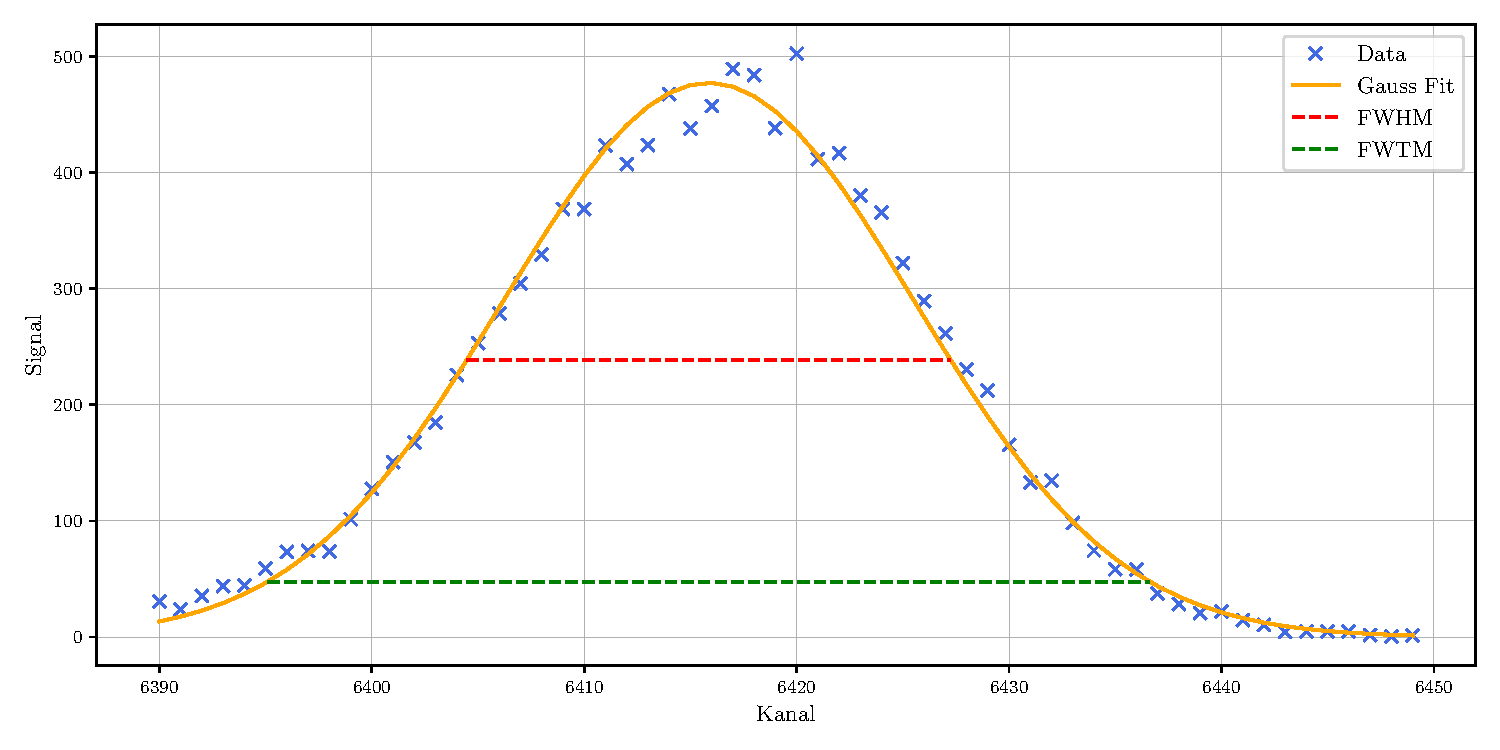
\includegraphics[width=\textwidth]{../plots/Caesium-Peak-6420.pdf}
  \caption{Vollenergiepeak des $^{137}\text{Cs}$-Strahlers.}
  \label{fig:photopeak}
\end{figure}
Für die Halbwertsbreite und die Zehntelwertsbreite ergeben sich mittels der gefitteten Gaußfunktion die Werte
\begin{align*}
  \text{FWHM} &= 22.77 \pm 0.16 \, \text{Kanäle} \\
  \text{FWTM} &= 41.51 \pm 0.29 \, \text{Kanäle} \, .
\end{align*}
Diese Werte können mittels der in \ref{sec:kalibrierung} bestimmten Kalibrierung in Energie umgerechnet werden.
Dabei ergeben sich die Werte
\begin{align*}
  \text{FWHM} &= 5.20 \pm 0.04 \, \si{\kilo\electronvolt} \\
  \text{FWTM} &= 9.48 \pm 0.07 \, \si{\kilo\electronvolt} \, .
\end{align*}
Das Verhältnis der Halbwertsbreite und Zehntelwertsbreite beträgt für die gefitteten Werte
\begin{equation*}
  \frac{\text{FWHM}}{\text{FWTM}} = 0.5467 \pm 0.0 \, .
\end{equation*}
und für die abgelesenen Werte
\begin{equation*}
  \frac{\Delta K_\text{FWHM}}{\Delta K_\text{FWTM}} = 0.5476 \, .
\end{equation*}

\subsubsection{Untersuchung des Compton-Effekts}
Der Inhalt der Photopeaks wurde durch die Integration der gefitteten Gaußfunktion bestimmt und ergibt sich zu $N_\text{Photo} = 11525.21 \,$ Impulsen.
Die Energie des Photopeaks lässt sich mittels der Kalibrierung \ref{sec:kalibrierung} bestimmen 
und beträgt $E_\text{Photo} = 1317.2446 \pm 0.0006 \, \si{\kilo\electronvolt}$.
Scheiinbar weicht der Wert von der Literaturenergie $E_\text{Lit} = 662 \, \si{\kilo\electronvolt}$ ab um ziemlich genau den Faktor 2 ab, 
worauf in der späteren Diskussion eingegangen wird.
Die Comptonkante und der Rückstreupeak können mittels der Photopeakenergie (hier wurde der Literaturwert verwendet) bestimmt werden \ref{eq:Compton} und belaufen sich auf
\begin{align*}
  E_\text{Compton Kante,1} &= 477.65 \, \si{\kilo\electronvolt} \\
  E_\text{Rückstreupeak,1} &= 184 \, \si{\kilo\electronvolt} \, .
\end{align*}
Wird die per Kalibrierung bestimmte Energie des Photopeaks verwendet, ergeben sich die Werte
\begin{align*}
  E_\text{Compton Kante,2} &= 1103.25 \, \si{\kilo\electronvolt} \\
  E_\text{Rückstreupeak,2} &= 214 \, \si{\kilo\electronvolt} \, .
\end{align*}
Aus diesen Energien lassen sich die Kanalnummern bestimmen, indem man die Kalibrierung invers anwendet.
Die Kanalnummer des Rückstreupeaks ist aus der Peakbestimmung \ref{fig:cs} bekannt.
Es ergeben sich die Kanalnummern
\begin{align*}
  K_\text{Compton Kante,2} &= 4980.4069 \pm 0.0025 \\
  K_\text{Rückstreupeak} &= 1868 \, .
\end{align*}
Die aus der Energie bestimmte Kanalnummer für den Rückstreupeak beträgt $K_\text{Rückstreupeak} = 955$.
Der Rückstreak, die Comptonkante und das Comptonkontinuum sind in der Abbildung \ref{fig:compton} dargestellt.
\begin{figure}[H]
  \centering
  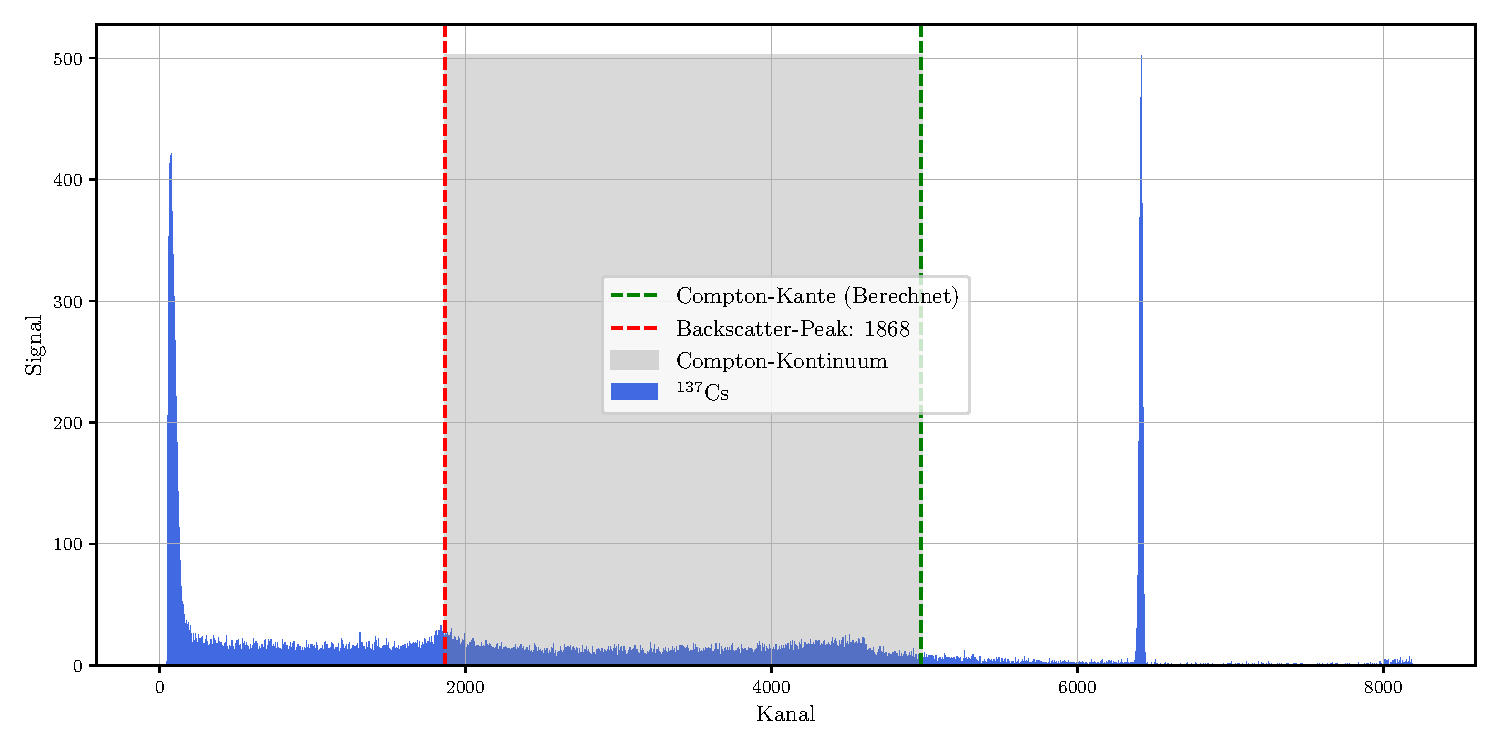
\includegraphics[width=\textwidth]{../plots/Caesium-Compton-Backscatter.pdf}
  \caption{Comptonkontinuum, Comptonkante und Rückstreupeak des $^{137}\text{Cs}$-Strahlers.}
  \label{fig:compton}
\end{figure}
Das Comptonkontinuum wurde durch eine lineare Regression der Form
\begin{equation}
  f(x) = a \cdot x + b
\end{equation}
gefittet.
Die Parameter der Regression betragen
\begin{align*}
  a &= -0.00183 \pm 0.00009 \\
  b &= 2.13 \pm 0.30 \, .
\end{align*}
Um den Einfluss des Rückstreupeaks auf das Comptonkontinuum zu minimieren wurde für die lineare Regression ein begrenzter Ausschnitt des Spektrums verwendet.
Die Regression ist in Abbildung \ref{fig:compton-Kontinuum} dargestellt.
\begin{figure}[H]
  \centering
  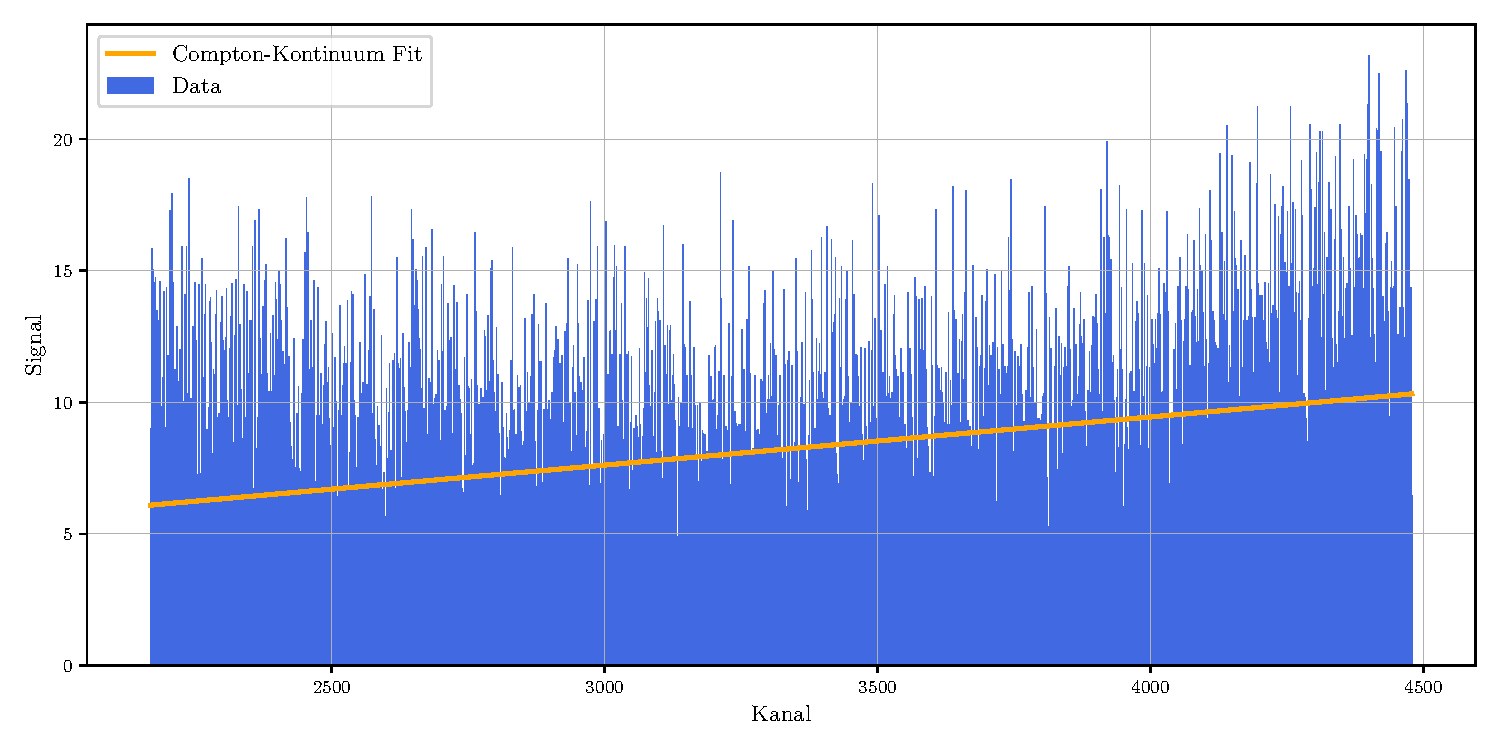
\includegraphics[width=\textwidth]{../plots/Caesium-Compton-Kontinuum.pdf}
  \caption{Lineare Regression des Comptonkontinuums.}
  \label{fig:compton-Kontinuum}
\end{figure}
Daraus lässt sich der Inhalt des Comptonkontinuums bestimmen und beträgt $N_\text{Compton-Kontinuum} = 26105.179 \, \text{Impulse}$.

\subsubsection{Bestimmung der Absoprionswahrscheinlichkeit}
Die Absorptionswahrscheinlichkeit $P$ lässt sich mit der Formel \ref{eq:Extinktion} bestimmen.
Die Extinktionskoeffizienten für den Compton-Effekt und den Photoeffekt sind 
\begin{align*}
  \mu_\text{Compton} &= 0.37 \, \si{\per\centi\meter} \\
  \mu_\text{Photo} &= 0.008 \, \si{\per\centi\meter} \, .
\end{align*}
Die Detektorlänge beträgt $d=3.9 \si{\centi\metre}$, somit ergeben sich die Absorptionswahrscheinlichkeiten
\begin{align*}
  P_\text{Compton} &= 76.4 \si{\percent} \\
  P_\text{Photo} &= 3.07 \si{\percent} \, .
\end{align*}
Demnach müsste der Inhalt des Comptonkontinuums um den Faktor $24.9$ höher sein als der des Photopeaks.
Die experimentell bestimmten Werte ergeben ein Verhältnis von
\begin{equation*}
  \frac{N_\text{Compton-Kontinuum}}{N_\text{Photo}} = \frac{26105.179}{11525.21}= 2.265 \, .
\end{equation*}

\subsection{Aktivitätsbestimmung von $^{133}\text{Ba}$} \label{sec:aktivität}
Die Aktivität der $^{133}\text{Ba}$-Probe wurde durch eine Messung des Spektrums bestimmt.
Die Dauer der Messung betrug $t = 3021 \, \si{\second}$.
Die Messdaten sind in der Abbildung \ref{fig:ba} dargestellt.
Die prominentesten Peaks wurden identifiziert und sind in der Tabelle \ref{tab:ba} aufgeführt.
\begin{figure}[H]
  \centering
  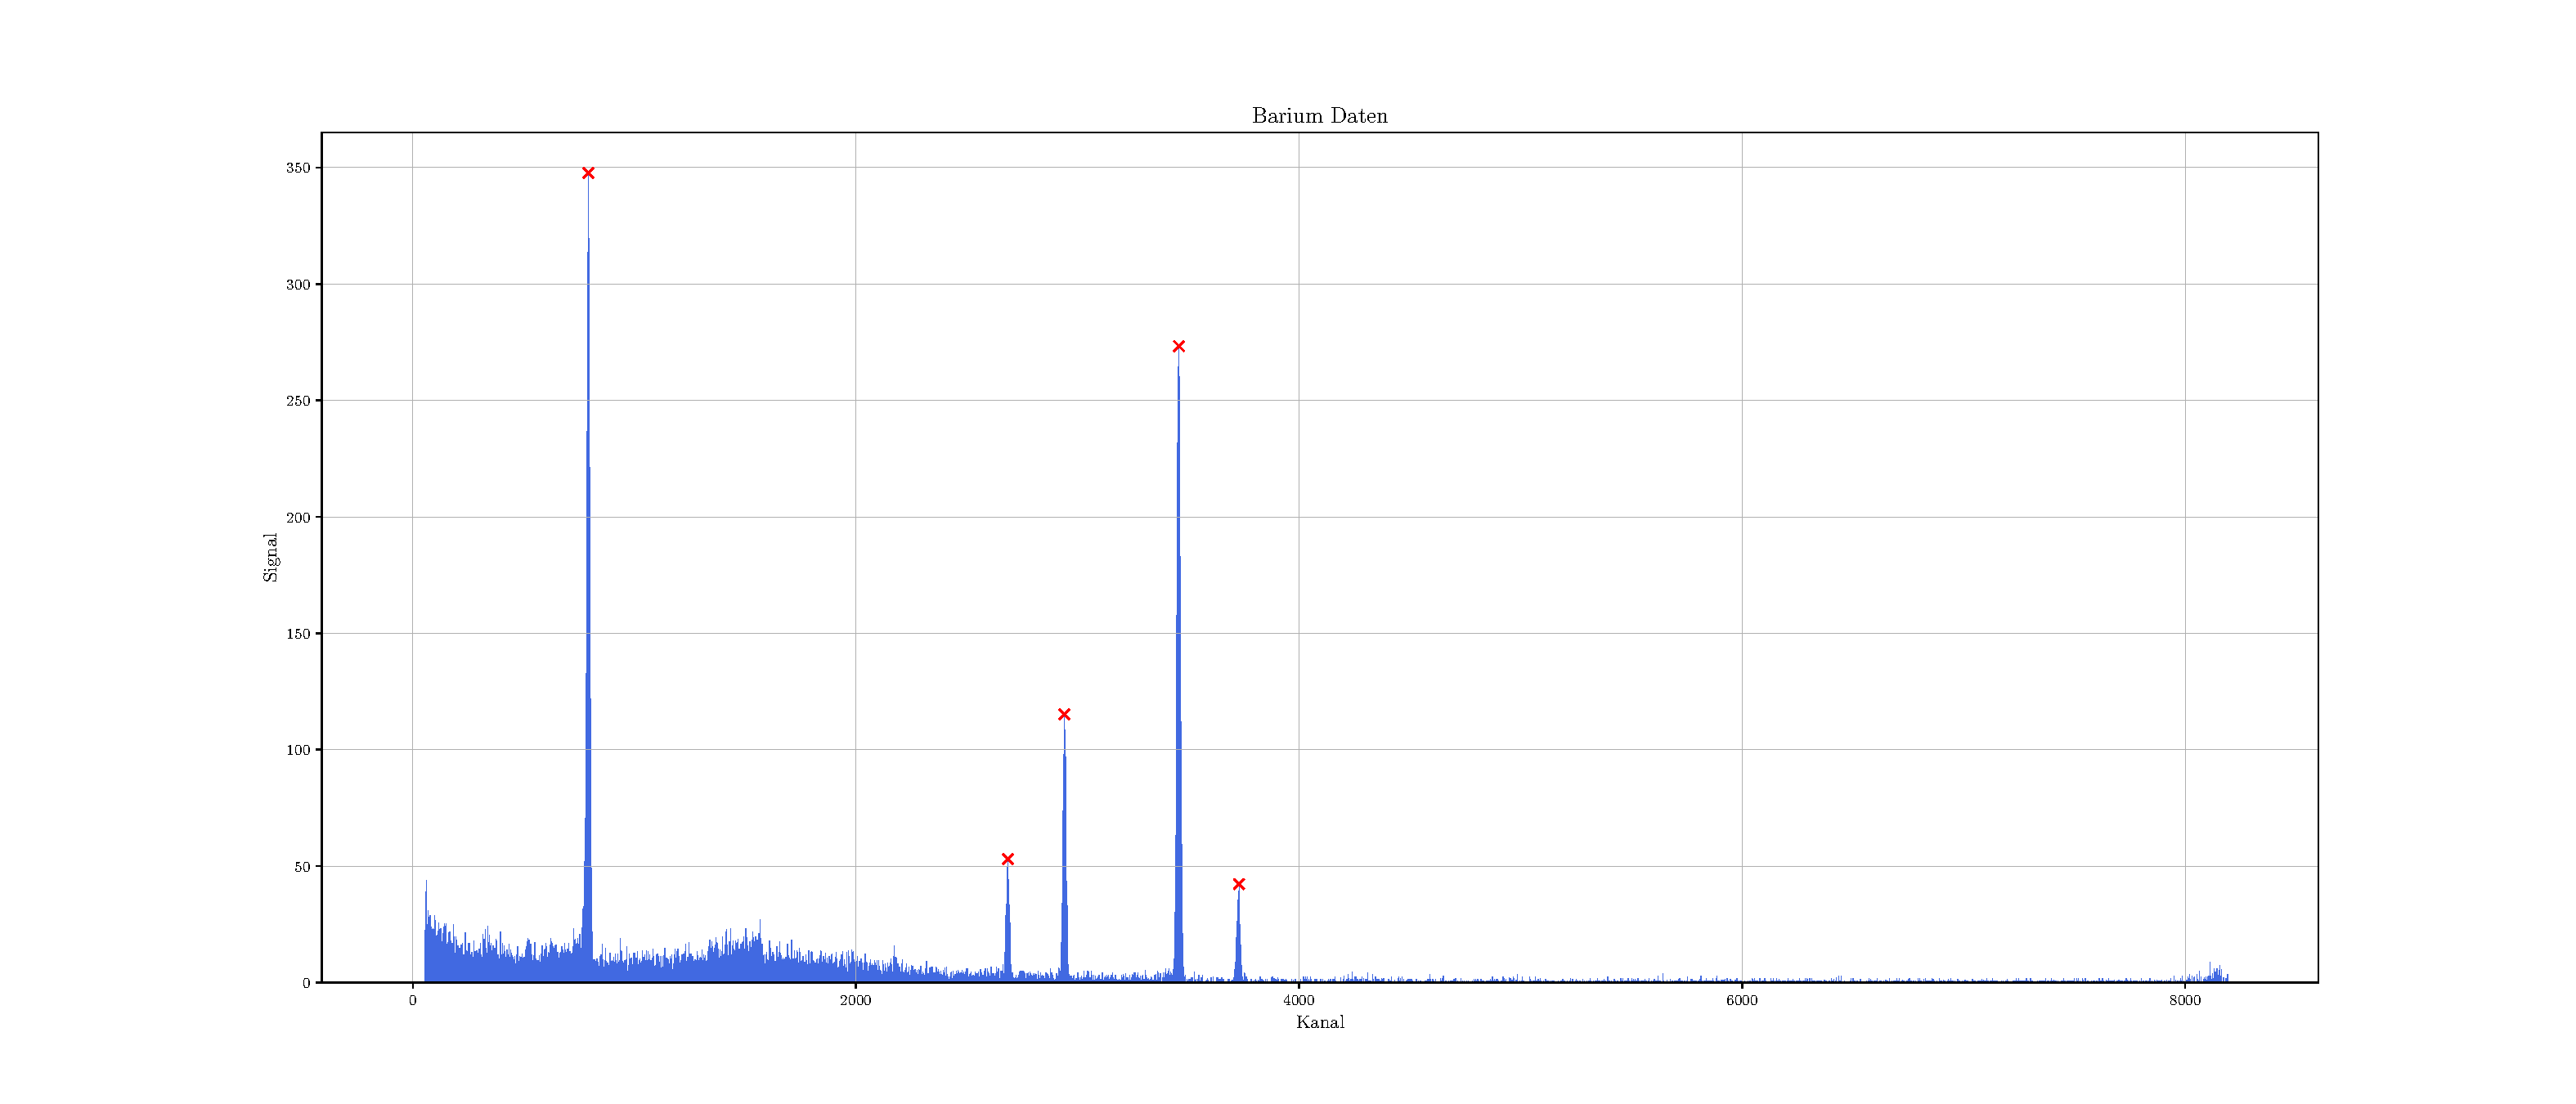
\includegraphics[width=\textwidth]{../plots/Barium.pdf}
  \caption{Spektrum des $^{133}\text{Ba}$-Strahlers.}
  \label{fig:ba}
\end{figure}
Die Aktivität der Probe soll im folgenden bestimmt werden.
Dafür wird die Gleichung \ref{eq:Q} nach der Aktivität umgestellt.
Für den Raumwinkel wird der bereits in \ref{sec:kalibrierung} bestimmte Wert verwendet.
Der Inhalt der Vollenergiepeaks wird durch eine Integration der Gaußfunktion bestimmt.
Die Effizienz $Q$ wird durch die nichtlineare Regression \ref{eq:Q-fit} bestimmt.
Dadurch ergeben sich die in der Tabelle \ref{tab:ba} aufgeführten Werte.
\begin{table}[H]
  \centering
  \caption{Energien \cite{Lara} und die Effizienz $Q$ der Vollenergiepeaks der $^{133}\text{Ba}$-Probe sowie die zugeordneten Kanäle, der bestimmte Inhalt und die daraus berechnete Aktivität.}
  \label{tab:ba}
  \begin{tabular}{c S[table-format=4.0] S[table-format=4.3] c S}
      \toprule {$E_\text{Lit} / \si{\kilo\electronvolt}$}  & {Kanal} & {Counts} & {$Q /\si{\percent}$} & {Aktivität $A/\si{\becquerel}$}\\
      \midrule
      80.9979 \pm 0.11  &793  &5580.537  &0.095 \pm 0.015   &35 \pm 6\\
      276.3989 \pm 0.12 &2685 &839.003   &0.021 \pm 0.004   &114 \pm 20\\
      302.8508 \pm 0.05 &2940 &1868.218  &0.0176 \pm 0.0032 &116 \pm 21\\
      356.0129 \pm 0.07 &3458 &5142.753  &0.0143 \pm 0.0026 &115 \pm 21\\
      383.8485 \pm 0.12 &3730 &607.006   &0.0130 \pm 0.0024 &104 \pm 19\\
      \bottomrule
  \end{tabular}
\end{table}
Aus den ermittelten Aktivitäten wird der Mittelwert und die Standardabweichung bestimmt.
Die Aktivität der $^{133}\text{Ba}$-Probe beträgt
\begin{equation*}
  A = 96.83 \pm 31.06 \, \si{\becquerel} \, .
\end{equation*}

\subsection{Nuklidbestimmung} \label{sec:nuklid}
Im letzten Versuchsteil soll die Zusammensetzung einer unbekannten Probe bestimmt werden.
Dafür wird das Spektrum der Probe gemessen und die prominentesten Peaks identifiziert.
Die Messdaten sind in der Abbildung \ref{fig:unbekannt} dargestellt.
Die Messung dauerte $t = 3427 \, \si{\second}$.
Wie auch bei den anderen Messungen wurde die durchgeführte Untergrundmessung abgezogen.
Zur Identifizierung wurde eine Nukliddatenbank \cite{Lara} herangezogen.
Die identifizierten Peaks und die zugehörigen Energien sind in der Tabelle \ref{tab:unbekannt} aufgeführt.
Da bei der Energiebestimmung des Photopeaks der Caesiumprobe ein systematischer Fehler aufgetreten ist, wird die Energie der Peaks der unbekannten Probe durch den aufgetretenen Faktor 2 geteilt.
\begin{figure}[H]
  \centering
  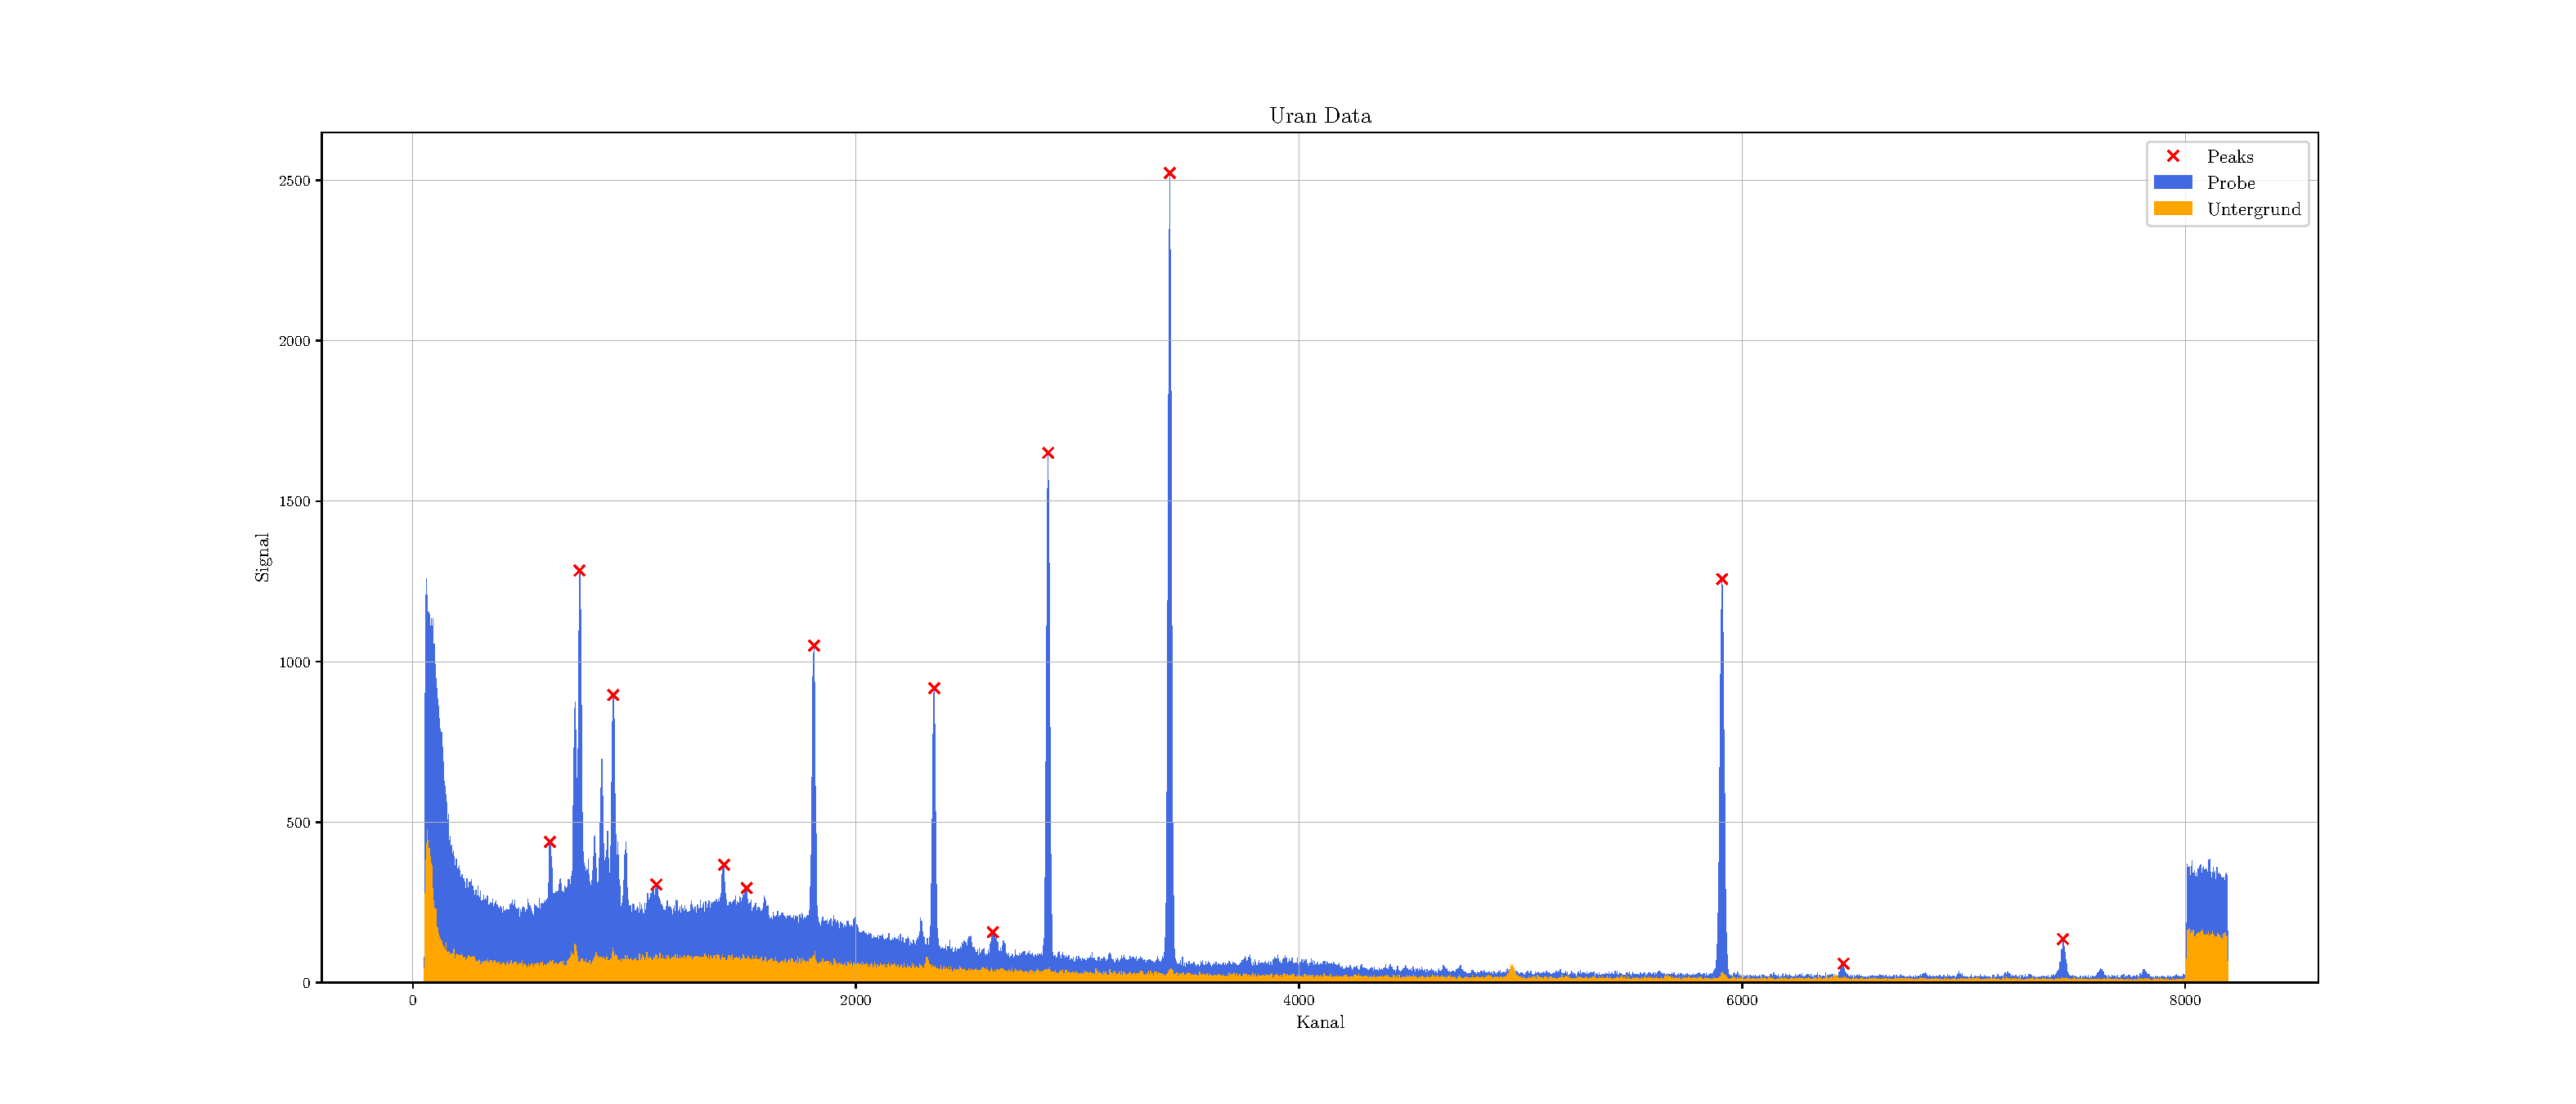
\includegraphics[width=\textwidth]{../plots/Uran.pdf}
  \caption{Spektrum der unbekannten Probe.}
  \label{fig:unbekannt}
\end{figure}

\begin{table}
  \centering
  \caption{Energien und die Kanäle der Vollenergiepeaks der unbekannten Probe sowie die zugeordneten Nuklide.}
  \label{tab:unbekannt}
  \begin{tabular}{S[table-format=4.0] S c S}
      \toprule {Kanal} & {$E / \si{\kilo\electronvolt}$} &  {Nuklid} & {$E_\text{Lit}$} \\
      \midrule
      620 &-3.54631\pm 0.0003  &         &  \\
      753 &11.63790\pm 0.0003  & Th-229  & 13.244 \\
      904 &28.87711\pm 0.0003  & Th-229  & 28.288 \\
      1100&51.25385\pm 0.0003  & Th-229  & 51.0 \pm 0.03\\
      1405&86.07478\pm 0.0003  & Th-229  & 86.3 \pm 0.03 \\
      1507&97.71981\pm 0.0003  & Th-229  & 97.37 \pm 0.04 \\
      1810&132.31242\pm 0.0003 & Th-229  & 132.1 \\
      2353&194.30510\pm 0.0003 & Th-228  & 191.351 \pm 0.11\\
      2618&224.55935\pm 0.0003 & Th-229  & 224.33 \pm 0.19 \\
      2868&253.10110\pm 0.0003 & Th-229  &255.91 \pm 0.02 \\
      3416&315.66462\pm 0.0003 & Th-229  & 315.39 \pm 0.13 \\
      5909&600.28295\pm 0.0003 & Pa-233  & 599.3  \pm 0.02 \\
      6458&662.96063\pm 0.0003 & Th-228  & 663.88 \pm 0.08\\
      7449&776.10013\pm 0.0003 & U-232   & 774.05 \pm 0.09 \\
      \bottomrule
  \end{tabular}
\end{table}

Ein mögliches Mutternuklid von $^{229}Th$ ist $^{233}U$, was zu der gelblichen Färbung der Probe passen würde.
Ein Tochternuklid von $^{233}Pa$ ist $^{233}U$.



